\documentclass[4paper]{article}
\usepackage[spanish]{babel}
%\usepackage[ansinew]{inputenc}
\usepackage[utf8x]{inputenc}
%\usepackage[utf-8]{inputenc}
%\usepackage[T1]{fontenc}
\usepackage{graphicx}
\usepackage{multicol}
%\usepackage{longtable}
%\usepackage{array}
%\usepackage{multirow}
%\usepackage[latin1]{inputenc}
%\inputencoding{latin1}

\renewcommand{\tablename}{Tabla}
\author{Manuel Molino Milla \and Luis Molina Garzón}
\title{\textbf{Programación}
\\Cadenas}
\date{\today}

\begin{document}
\maketitle
%\tableofcontents
%\setlongtable 


\section*{Ejercicio 1}
Crea una clase denominada \emph{PalabraLeida}, que tenga como único atributo un \emph{String} denominado \emph{valor} y que contenga los siguientes métodos:
\begin{itemize}
\item NumeroDeLetras()
\item EmpiezaPorVocal()
\item AcabaEnVocal()
\item NumeroDeVocales()
\item ContieneH()
\item EsUnPalindromo()
\item SonIguales(String palabra):boolean (sin tener en cuenta mayúsculas o minúsculas)
\end{itemize}
Una palabra es un palíndromo si al leerla de izquierda a derechas es la misma palabra leida en sentido contrario, ejemplo \emph{reconocer, rotor, salas, seres, somos}.\\
Posteriormente crea una clase denominada \emph{TestPalabraLeida} que compruebe el funcionamiento de dicha clase y lea la palabra mediante la clase Scanner.\\ Para comprobar el funcionamiento del método \emph{SonIguales(String palabra):boolean} utiliza los argumentos del programa principal para obtener el parámetro \emph{String} de dicho método.\\
Genera la documentación de la clase \emph{PalabraLeida} y el diagrama UML de la misma.\\
Crea un fichero jar ejecutable que compruebe el funcionamiento del \emph{TestPalabraLeida}

\section*{Ejercicio 2}
Crea una nueva clase denominada \emph{ClaveSegura} que tenga como único atributo un \emph{String} denominado clave. Puedes usar un \emph{constructor} o un \emph{setter} para la inicialización de dicho atributo.\\
Dicha clase contará con un método que se llame \emph{esClaveSegura}. Una clave es segura si cumple los siguientes requisitos:
\begin{itemize}
\item Tenga al menos 8 caracteres.
\item Tenga al menos una letra en minúscula.
\item Tenga al menos una letra en mayúscula.
\item Contenga al menos un número.
\item Tenga al menos un carater no alfanumérico.
\end{itemize}
Posteriormente crea una clase \emph{TestClaveSegura} que genere de forma aleatoria clave de longitud aleatoria (entre 0 y fuenteCaracteres.length()-1), muestre por pantalla dicha clave e indique si es segura o no.\\
Para obtener los caracteres que forman la clave se usará los caracteres del siguiente String: 
\begin{verse}
String final FUENTE\_CARACTERES = ''aAbBcCdDeEfFgGhHiIjJkKlLmMnNñÑoOpPqQrRsStTuUvVwWxXyYzZ0123456789¿?()=@.:,;!¡\&\{\}'';
\end{verse}
Genera la documentación de la clase \emph{ClaveSegura} y el diagrama UML de la misma.
\\
Crea un fichero jar ejecutable que compruebe el funcionamiento del \emph{TestClaveSegura}


\section*{Ejercicio 3}
Queremos leer los datos de un fichero de texto pero sin tener que usar las clase que aporta java en relación a entrada y salida, para esto realizaremos el siguiente comando:
\begin{verbatim}
cat nombres_mujer.txt | java Programa
\end{verbatim}
En el caso de windows cambia el comando cat por type.\\
El programa no va a usar el paradigma de POO y deberá hacer lo siguiente:
\begin{itemize}
\item Usaremos la clase Scanner para realizar la lectura.
\item Indicar cuantas palabras ha leido.
\item Crear dos listas una con aquellos nombres que empiezan por A y otra para aquellas palabras que no acaben en vocal. Posteriormente las mostramos por pantalla.
\item Crea otra dos listas para guardar las palabras con mas y con menos letras. Ambas listas contendran String con el mismo tamaño. Posteriormente mostramos por pantalla ambas listas.
\item En el caso que pasemos un argumento al programa, el programa no debe realizar nada de lo anterior y lo que debe hacer es compruebar si dicho argumento es un nombre que aparece en el fichero y nos diga por tanto que existe, o bien que nos sugiera nombre que empiezan por la dos primeras letras que el parámetro pasado.
\end{itemize}
\newpage

\section*{Ejercicio 4}
Igual que en el ejercicio anterior, lee el fichero \emph{contitucion.txt.} Guarda cada palabra en un \emph{ArrayList}. Posteriormente crea un \emph{StringBuilder} en el que vas a añadir quinientos \emph{String} del \emph{ArrayList} inicial, la elección de la posición del \emph{String} se hace de forma aleatoria entre los número 0 y el tamaño del \emph{ArrayList} (puede haber repeticiones de palabras o posiciones). Todo esto lo realizas en una clase denominada \emph{TestConstitucion.java}.\\
Posteriormente implementa la clase UtilidadesStrig.java de acuerdo a su \emph{diagrama UML}.\\
En la clase \emph{TestConstitucion.java} comprueba el funcionamiento de la clase anterior.\\
Para contar el número de articulos o preposiciones, puedes convertir el \emph{String} en un array de \emph{String} mediante el método \emph{splice} de la clase \emph{String}.\\
Genera la documentación de la clase \emph{UtilidadesString.java}
\begin{figure}
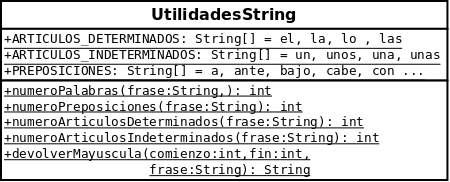
\includegraphics[scale=0.6]{utilidades.png}
\end{figure}
\end{document}
